\documentclass[11pt]{article}
\usepackage{graphicx}

\begin{document}

\title{Homework 1}
\date{}
\author{Colt Bradley}
\maketitle

\section{Text}
This section is an example of basic text using \textbf{LaTeX}. It`s {\em very} important to understand that using LaTeX is different than Microsoft word. You must format text correctly.

\section{Equation}

Here`s an example of an inline equation: ``we use $ax^2 +bx+c=0$ as the standard form for a quadratic equation."

\begin{equation}
\int \left( \frac{(x-1)}{\sqrt{x^2 +1}} + \sqrt{x^2 +1} \right) dx = \left( 1 + \frac{x}{2} \right) \sqrt{x^2 +1}- \frac{1}{2} \arcsin x +C \label{crazyequation}
\end{equation}

As you can see, the equation above (\ref{crazyequation}) is not inline; it requires different formatting.

\section{Graphics}

Adding a graphic is a bit annoying, as LaTeX throws it wherever it likes. However, this does make sense after closer inspection. It's on the next page.

\begin{figure}
\centering
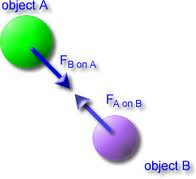
\includegraphics[scale=.5]{N3L.jpg}
\caption{Here's the graphic from the lesson}
\end{figure}

\end{document}
